%%This is a very basic article template.
%%There is just one section and two subsections.
\documentclass{article}

\usepackage{a4wide}
\usepackage{listings}
\usepackage{float}
\usepackage{listings}
\usepackage{graphicx}
\usepackage{epstopdf}

\lstset{ %
breaklines=true,
language=R
}

\begin{document}

\title{Probability and Statistics for Data Analysis\\Assignment 2}
\author{Charalampos Kaidos}

\maketitle

\section*{Exercise 7}

In a lottery we have 30 balls numbered 1 - 30 that are well mixed in an urn. We
draw without replacement 5 balls from the urn and a ticket is winning when it
guessed all 5 numbers. In the spreadsheet named Lottery\_Data of the file
Assignment\_2\_data.xlsx (available on e-class assignments site) we provide the
most recent 10,000 draws from the urn.  Using these data answer the following
questions:

First we read the data. I used the xlsx library to read the excel file, then
picked the sheet and stored it in csv format to allow easier access and storage
to CVS. I use these csvs to load the data.

\begin{lstlisting}
lottery_data <- read.csv("lottery_data.csv", header = FALSE)
\end{lstlisting}

\begin{enumerate}
  \item Is this a fair lottery?  Provide as much of graphical and numerical
  evidence as you can for or against this argument.
  
  First we will tranform the data; we will concatenate all the columns to one.
  This will allow easier manipulation of the data. Then we will treat the data
  as factors. They are factors as the problem states that there are 30 different
  balls. Finally we will make a barplot of frequencies for each ball
  (figure~\ref{fig:barplot}, p.~\pageref{fig:barplot}).
  
  \begin{lstlisting}
single_file <- stack(lottery_data)[1]
single_file <- factor(single_file[[1]])
frequencies <- summary(single_file)
barplot(frequencies, xlab = "Balls", ylab = "Times drawn", main = "Frequency diagram of lottery balls drawn in 10,000 draws", col=terrain.colors(30))
  \end{lstlisting}
    
  \begin{figure}[H]
  \centering
  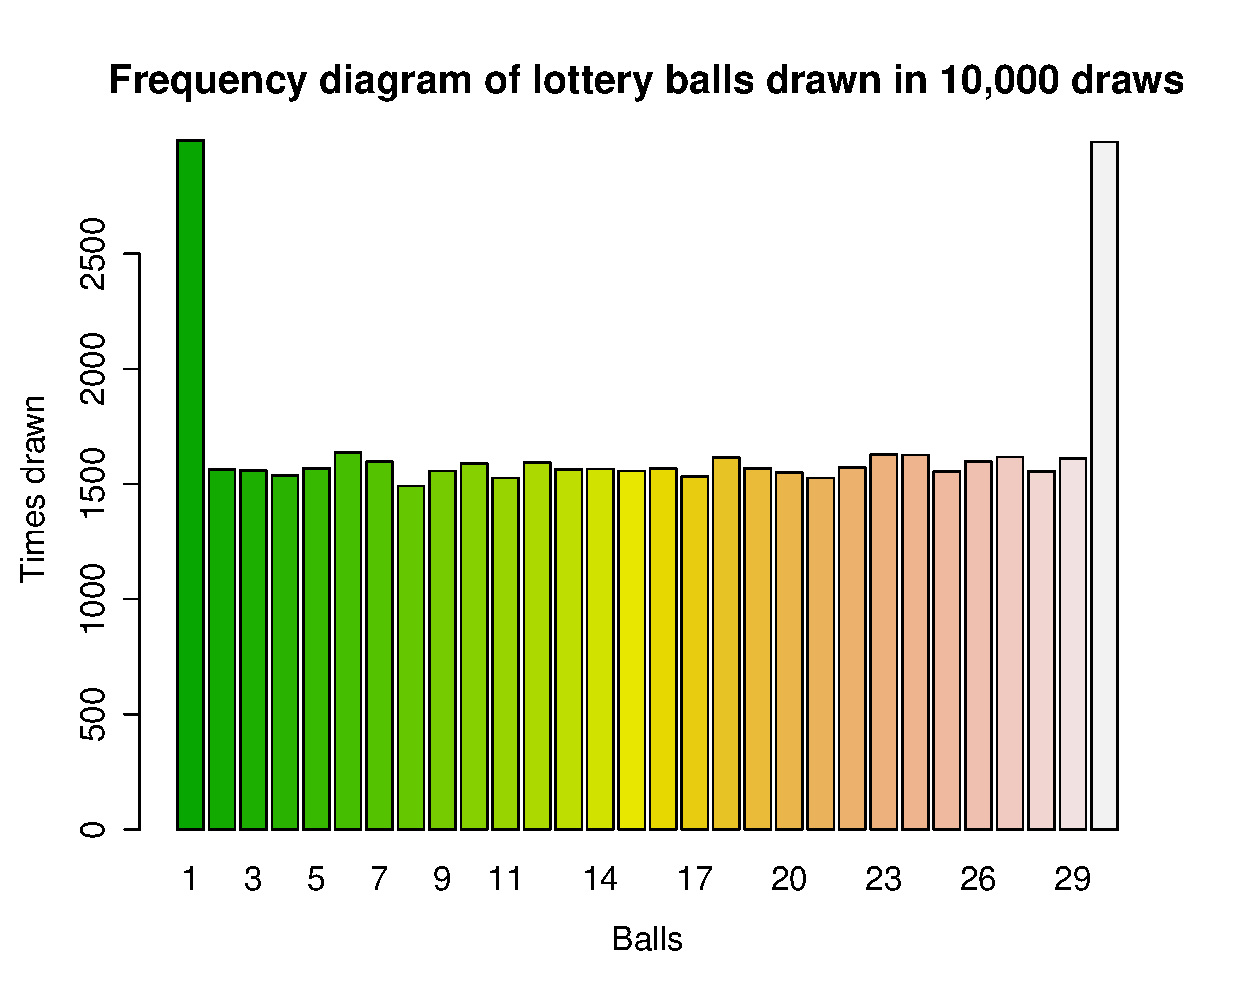
\includegraphics[scale=0.6]{barplot.eps}
  \caption{Barplot}
  \label{fig:barplot}
  \end{figure}
  
  
  That indeed is strange and a strong indication that the lottery is not fair as
  it seems that the balls numbered 1 and 30 are drawn about twice as much as the
  other balls.
  We expect that each ball will have equal probability to be drawn at a lottery.
  The frequencies indicate otherwise. Nevertheless we will try to test this
  hypothesis using the chi-squared test and setting equal probabilities for all
  balls.
  
  \begin{lstlisting}
> chisq.test(frequencies)

	Chi-squared test for given probabilities

data:  frequencies
X-squared = 2267.9, df = 29, p-value < 2.2e-16
  \end{lstlisting}
  
  The chi-squared test rejects the hypothesis that the draws are from a uniform
  distribution; that is that the balls have equal probabilities in this lottery.
  Actually the probability that we will get 10,000 draws with more bias 
  than these from a fair lottery is less than $2.2*10^{-16}$.
  We can conclude that the lottery is not fair.
  
  \item If you would play this lottery, would you have some favorable number(s)?
  
  If we were to play this lottery we would definetly choose numbers 1 and 30.
  They have about twice as much probability to be drawn compared to other
  numbers.
  
  \item How your answers in the previous two questions would change if you use
  only the first 100 recorded draws? How about if you used only the first 1,000
  recorded draws?
  
  If we were to use only the first 100 draws we would get a barplot like the one
  in figure~\ref{fig:barplot100} (p.~\pageref{fig:barplot100}).
  
  \begin{lstlisting}
single_file_100 <- stack(lottery_data[1:100,])[1]
single_file_100 <- factor(single_file_100[[1]])
frequencies_100 <- summary(single_file_100)
barplot(frequencies_100, xlab = "Balls", ylab = "Times drawn", main = "Frequency diagram of lottery balls drawn in 100 draws", col=terrain.colors(30))
  \end{lstlisting}
  
  \begin{figure}[H]
  \centering
  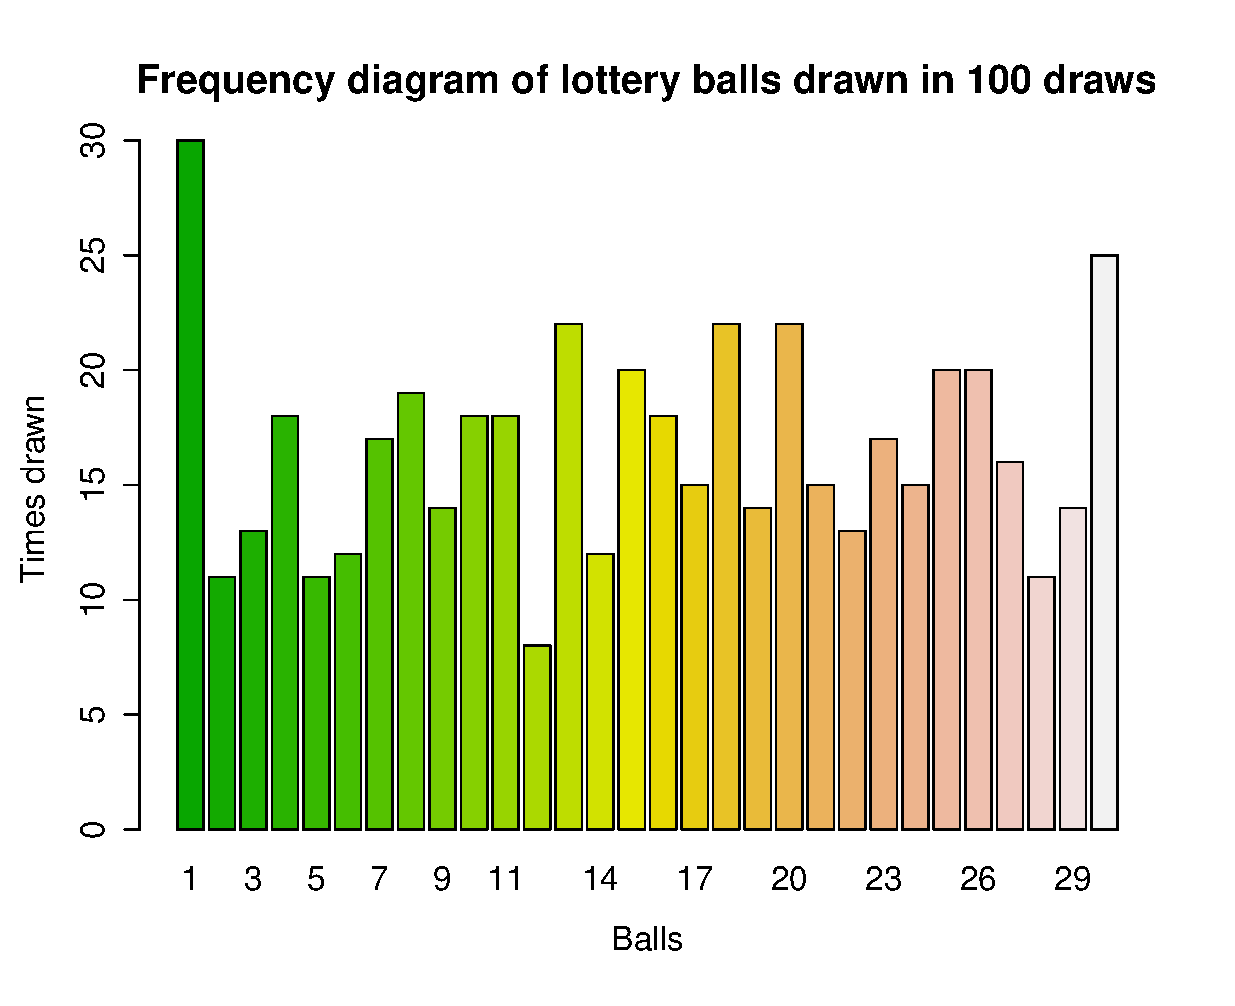
\includegraphics[scale=0.6]{barplot100.eps}
  \caption{Barplot for 100 first draws}
  \label{fig:barplot100}
  \end{figure}
  
  We can see that the problem is not shown clearly here. The frequencies for all
  balls are rather small ranging from 8 to 30 and we cannot argue that the
  probabilities are not equal. The chi-squared test confirms this:
  
  \begin{lstlisting}
> chisq.test(frequencies_100)

	Chi-squared test for given probabilities

data:  frequencies_100
X-squared = 39.04, df = 29, p-value = 0.1009
  \end{lstlisting}

  When we use the first 1,000 draws the frequencies barplot becomes like in
  figure~\ref{fig:barplot1000} (p.~\pageref{fig:barplot1000}). Here the bias
  towards balls 1 and 30 is clear.
  
  \begin{figure}[H]
  \centering
  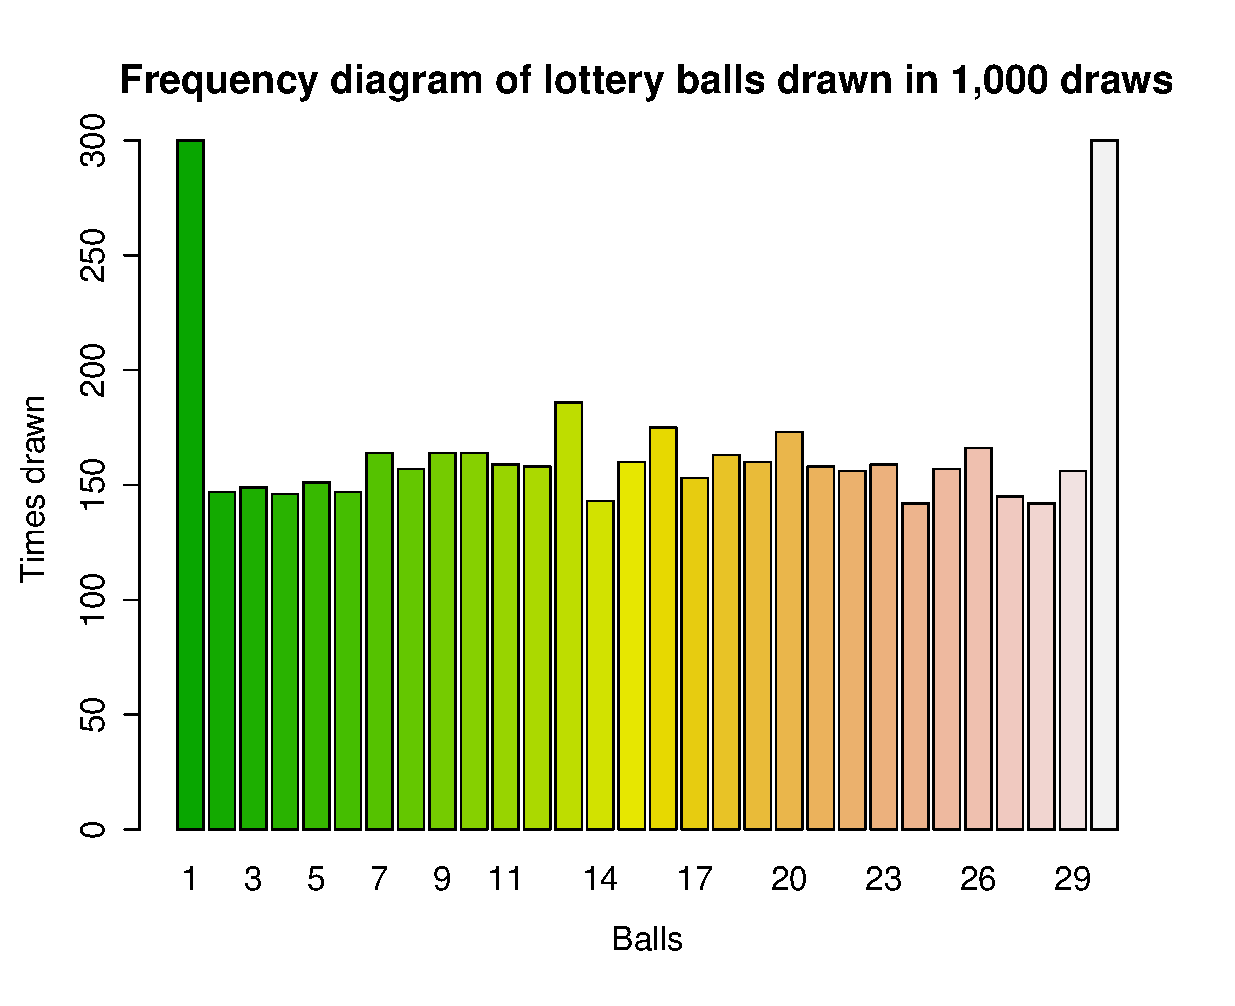
\includegraphics[scale=0.6]{barplot1000.eps}
  \caption{Barplot for 1000 first draws}
  \label{fig:barplot1000}
  \end{figure}
  
  The chi-squared test confirms this too. 1000 draws are enough to make sure
  that the lottery is not fair.
  
  \begin{lstlisting}
> chisq.test(frequencies_1000)

	Chi-squared test for given probabilities

data:  frequencies_1000
X-squared = 246.22, df = 29, p-value < 2.2e-16
  \end{lstlisting}
  
  \end{enumerate}

\end{document}
